\part{Keypoint Detection}\label{part:Keypoint detection}

正如上一章所讲,因为我们希望提取到的局部特征具有尺度不变性,所以既要找局部特征所在位置,还要确定它们的尺度。\lpl 已经被说明能够很好地完成上述任务,但它还不是最优的。本章将介绍\sift 是如何优化的,以及程序在实现关键点检测时的一些细节。

\section{构造高斯差分金字塔}

\sift 注意到一个明显的问题是当\lpl 尺度越来越大$\sigma$时,卷积窗口$w$也会越来越大(一般认为$w\approx 2\times\lceil 3\sigma\rceil + 1$),计算消耗也会越来越明显。为了解决这一问题,\sift 指出可以采用\DoG 完成如下近似:
\begin{equation}
	\eqnmarkbox[emph2]{dog}{G(x,y,k\sigma) - G(x,y,\sigma)} \approx (k-1)\eqnmarkbox[emph2]{log}{\sigma^2\nabla^2 G}
	\label{equ: DoG and LoG}
\end{equation}
\annotate[]{below}{dog}{\DoG}
\annotate[]{below}{log}{scale-normalized \lpl}

\begin{marginfigure}
	\centering
	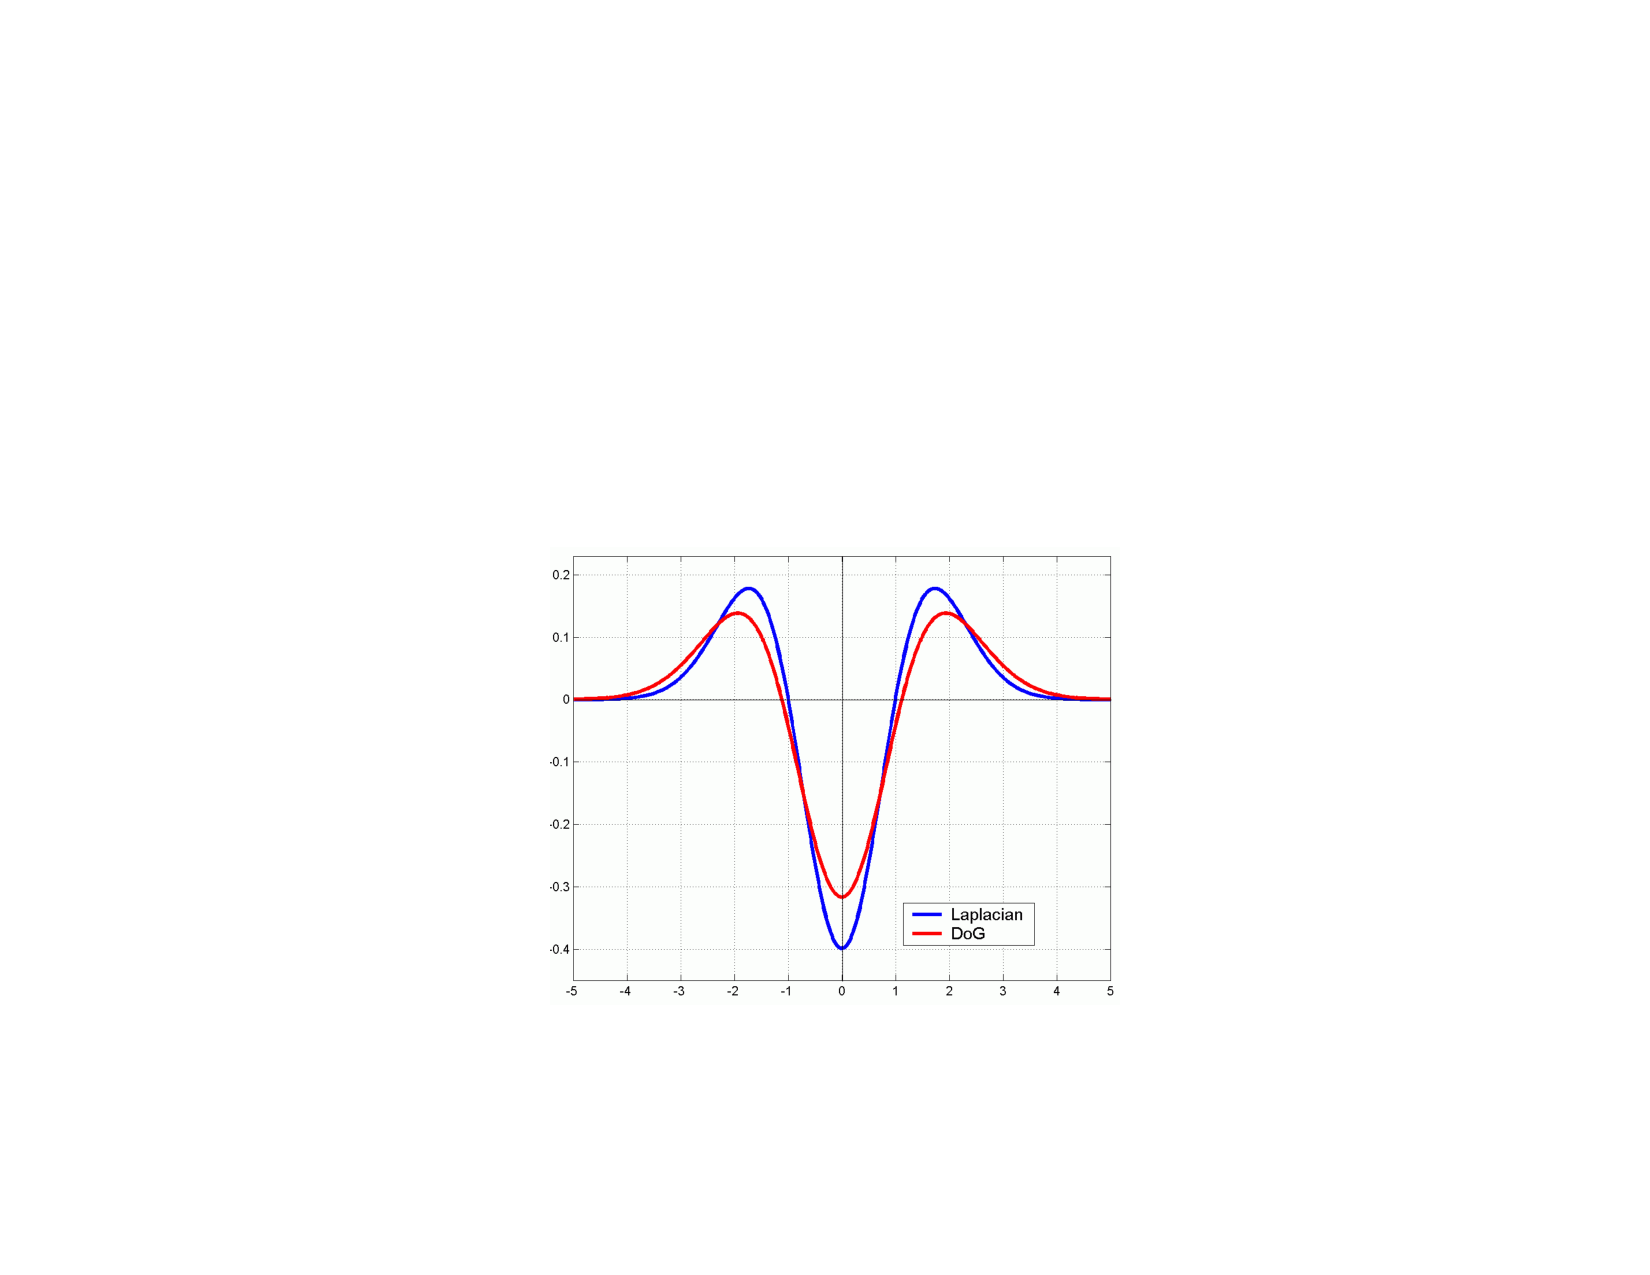
\includegraphics[width=\textwidth]{fig/Approximate LoG with a difference of Gaussians.pdf}
	\caption{Approximate LoG with a difference of Gaussians}
\end{marginfigure}

上式表明,在不考虑尺度因子$k-1$的情况下,\DoG 约等于尺度归一化后的\lpl。利用\DoG 近似的好处是,由高斯卷积的性质,大的高斯核($G(x,y,k\sigma)$)可以拆成两个小高斯核的卷积(\thmref{thm: gaussian convolution}),即要想获得方差更大高斯滤波,只需要在小方差高斯滤波的结果上继续进行一个小方差高斯滤波即可。
\begin{theorem}
	\label{thm: gaussian convolution}
	用两个方差分别为$\sigma^2_1$和$\sigma^2_2$的高斯核与图像进行连续的卷积滤波操作,该过程等价于直接用一个方差为$\sigma^2_1 + \sigma^2_2$的高斯核与图像进行一次卷积滤波操作。即:
	\begin{equation*}
		G(x, y, \sigma^2_1 + \sigma^2_2) = G(x, y, \sigma^2_1) \ast G(x, y, \sigma^2_2)
	\end{equation*}
\end{theorem}

于是$G(x,y,k\sigma)$可以表示为:
\begin{equation}
	G(x,y,k\sigma) = G(x,y,\sqrt{k^2 - 1}\sigma) \ast G(x,y,\sigma)
	\label{equ: gaussian convolution}
\end{equation}
这是提升\DoG 图像金字塔创建效率的有效方法。

\begin{figure}[H]
	\centering
	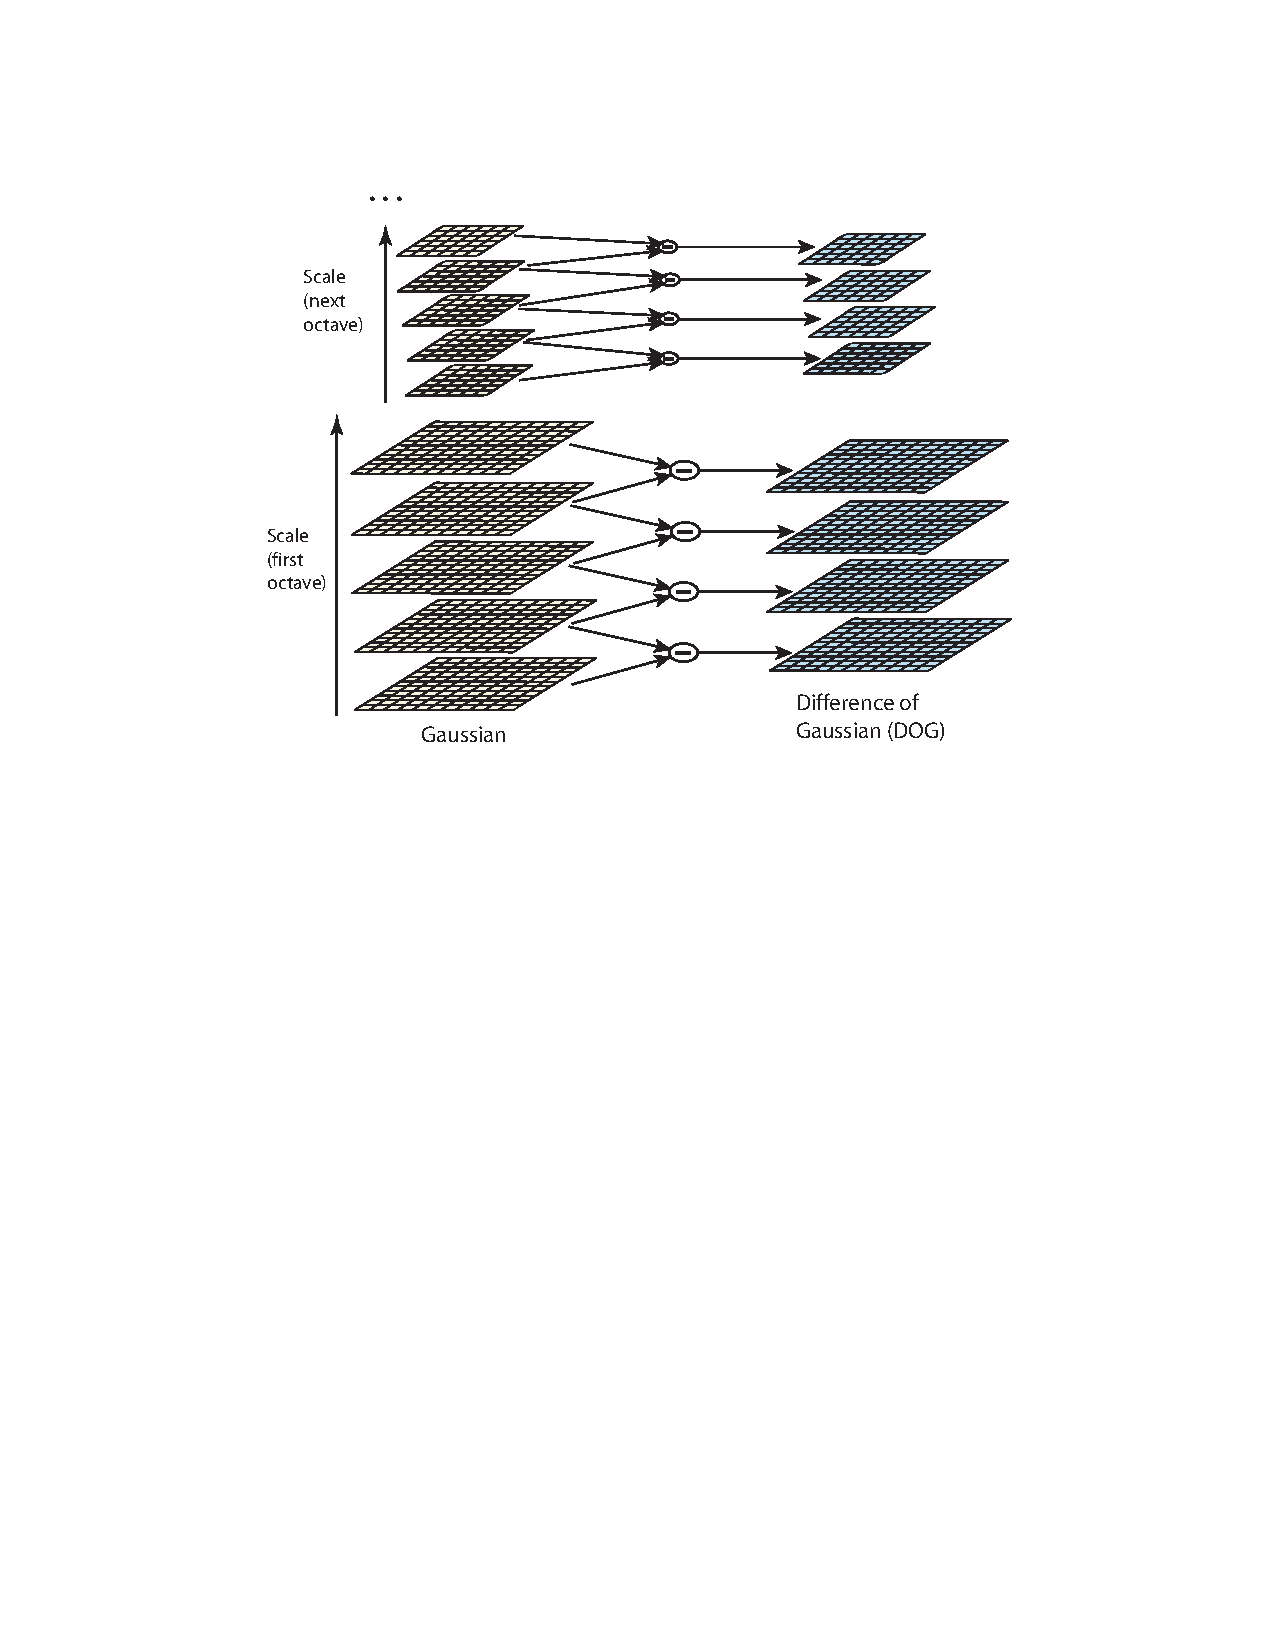
\includegraphics[width=.9\textwidth]{fig/construction of DoG.pdf}
	\caption{\DoG 图像金字塔}
	\label{fig: DoG Pyramid}
\end{figure}

\DoG 图像金字塔的结构如\figref{fig: DoG Pyramid},它基本由如下三个参数确定:
\begin{itemize}
	\item 每一个\octave 中包含的尺度个数$S$;
	\item \octave 的个数$O$;
	\item 标准差基本值$\sigma_0$。
\end{itemize}

如\figref{fig: DoG Pyramid}所示,在每一个\octave 的高斯金字塔(左侧)内一共需要进行$S+3$次高斯操作,高斯核的标准差从下往上依次扩大$k=2^{1/S}$倍(这样设置能够确保待检测的尺度在每个\octave 之间刚好连续),相邻两层相减就得到了右侧的\DoG 。通过直接对一个\octave 的高斯金字塔的第$S$层进行两倍下采样,获得下一个\octave 的最底层。下面是构建\DoG 图像金字塔的步骤:
\begin{enumerate}
	\item 加载灰度图像,对图像进行灰度归一化,也可缩小图像以加快处理效率;
	\item 对于索引$s=[0, 1, \ldots, S+2]$,用标准差$k^s\sigma_0$对图像进行高斯模糊。这里可以采用\equref{equ: gaussian convolution}介绍的方法提高效率,每一层直接在上一层的基础上进行模糊;
	\item 相邻的两张高斯模糊图像做差得到\DoG,每三层\DoG 就可以叠放成\figref{fig:Scale-space blob detector}所示的3D张量;
	\item 重复2-3步以最终得到$O$个\octave 。后面每个\octave 的最底层高斯模糊图像可以直接从上一\octave 的第$S$层经两倍下采样获得。
\end{enumerate}

\section{定位关键点}

在上一章\secref{sec:图像尺度空间}中提到,\emph{关键点}即在\DoG 尺度空间比它的领域都要大的极值点。搜索关键点的过程同时也需要进行非极大值抑制,因为图像中的相邻像素在\DoG 中的响应很可能相同,这会对后续特征点匹配的稳定性造成影响。同时还可以设置阈值,去除对比度低的点,因为这些点可能来自噪声。下面是程序中搜索定位关键点的步骤:
\begin{enumerate}
	\item 抑制所有响应小于阈值$C$的点;
	\item 将每个\octave 中的$S+2$个\DoG 叠成一个$H\times W\times (S+2)$的张量,比较张量中每一个位置和它$26(8+9+9)$个邻域之间的大小关系。如果一个位置比它邻域都要大,则它是一个关键点。忽略\DoG 金字塔最底层和最高层中检测到的关键点,即只在张量的$[\cdot, \cdot, 1]\sim [\cdot, \cdot, S]$部分提取关键点。
	\item 对每个\octave 重复上述过程。
\end{enumerate}
